% -*- latex -*-

%%%%%%%%%%%%%%%%%%%%%%%%%%%%%%%%%%%%%%%%%%%%%%%%%%%%%%%%%%%%%%%%%%%%%%%%%%%%%
% This beginning part of the preamble is psecific to the IEEEtran document
% class.

\documentclass[conference]{IEEEtran}

%% \author{
%%   \IEEEauthorblockN{Kenneth~Moreland}
%%   \IEEEauthorblockA{Sandia National Laboratories\\
%%     Albuquerque, NM 87185-1326\\
%%     Email: kmorel@sandia.gov}
%%   \and
%%   \IEEEauthorblockN{Others}
%%   \IEEEauthorblockA{Cool Group\\
%%     Somewhere, WQ 12341\\
%%     Email: person@myspace.com}
%% }

\author{
  \IEEEauthorblockN{
    Kenneth~Moreland\IEEEauthorrefmark{1}
  }
  \IEEEauthorblockA{
    \IEEEauthorrefmark{1}Sandia National Laboratories,
    Albuquerque, NM 87185-1326}
}

% for over three affiliations, or if they all won't fit within the width
% of the page, use this alternative format:
%
%\author{\IEEEauthorblockN{Michael Shell\IEEEauthorrefmark{1},
%Homer Simpson\IEEEauthorrefmark{2},
%James Kirk\IEEEauthorrefmark{3},
%Montgomery Scott\IEEEauthorrefmark{3} and
%Eldon Tyrell\IEEEauthorrefmark{4}}
%\IEEEauthorblockA{\IEEEauthorrefmark{1}School of Electrical and Computer Engineering\\
%Georgia Institute of Technology,
%Atlanta, Georgia 30332--0250\\ Email: see http://www.michaelshell.org/contact.html}
%\IEEEauthorblockA{\IEEEauthorrefmark{2}Twentieth Century Fox, Springfield, USA\\
%Email: homer@thesimpsons.com}
%\IEEEauthorblockA{\IEEEauthorrefmark{3}Starfleet Academy, San Francisco, California 96678-2391\\
%Telephone: (800) 555--1212, Fax: (888) 555--1212}
%\IEEEauthorblockA{\IEEEauthorrefmark{4}Tyrell Inc., 123 Replicant Street, Los Angeles, California 90210--4321}}

% End of IEEEtran-specific portion of the preamble.
%%%%%%%%%%%%%%%%%%%%%%%%%%%%%%%%%%%%%%%%%%%%%%%%%%%%%%%%%%%%%%%%%%%%%%%%%%%%%


\usepackage{amsfonts}
\usepackage{amssymb}
\usepackage{amsmath}
\usepackage{booktabs}
\usepackage{graphicx}
\usepackage{varioref}
\usepackage{fancyvrb}
\usepackage{ifthen}
\usepackage{cite}
\usepackage{subfig}
\usepackage{xspace}
\usepackage[pdfborder={0 0 0}]{hyperref}
\usepackage{verbatim}

\usepackage{color}
\definecolor{yellow}{rgb}{1,1,0}
\definecolor{black}{rgb}{0,0,0}
\definecolor{ltcyan}{rgb}{.75,1,1}
\definecolor{red}{rgb}{1,0,0}
\definecolor{gray}{rgb}{.6,.6,.6}
\definecolor{darkred}{rgb}{0.5,0,0}
\definecolor{darkgreen}{rgb}{0,0.5,0}

% Cite commands I use to abstract away the different ways to reference an
% entry in the bibliography (superscripts, numbers, dates, or author
% abbreviations).  \scite is a short cite that is used immediately after
% when the authors are mentioned.  \lcite is a full citation that is used
% anywhere.  Both should be used right next to the text being cited without
% any spacing.
\newcommand*{\lcite}[1]{~\cite{#1}}
\newcommand*{\scite}[1]{~\cite{#1}}

\newcommand{\etal}{et al.}

\newcommand{\insitu}{\it in situ\xspace}
\newcommand{\intransit}{\it in transit\xspace}

\newcommand*{\keyterm}[1]{\emph{#1}}

\newcommand{\fix}[1]{{\color{red}\textsc{[#1]}}}

% Avoid putting figures on their own page.
\renewcommand{\textfraction}{0.05}
\renewcommand{\topfraction}{0.95}
\renewcommand{\bottomfraction}{0.95}

% Make sure this is big enough so that only big figures end up on their own
% page but small enough so that if a figure does have to be on its own
% page, it won't push everything to the bottom because it's not big enough
% to have its own page.
\renewcommand{\floatpagefraction}{.75}

\title{Oh, \$\#*@! Exascale! The Effect of Emerging Architectures on
  Scientific Discovery}

% I hacked up IEEEtran.cls to support a teaser for conference papers.
\newcommand{\teaser}{
  \centering
  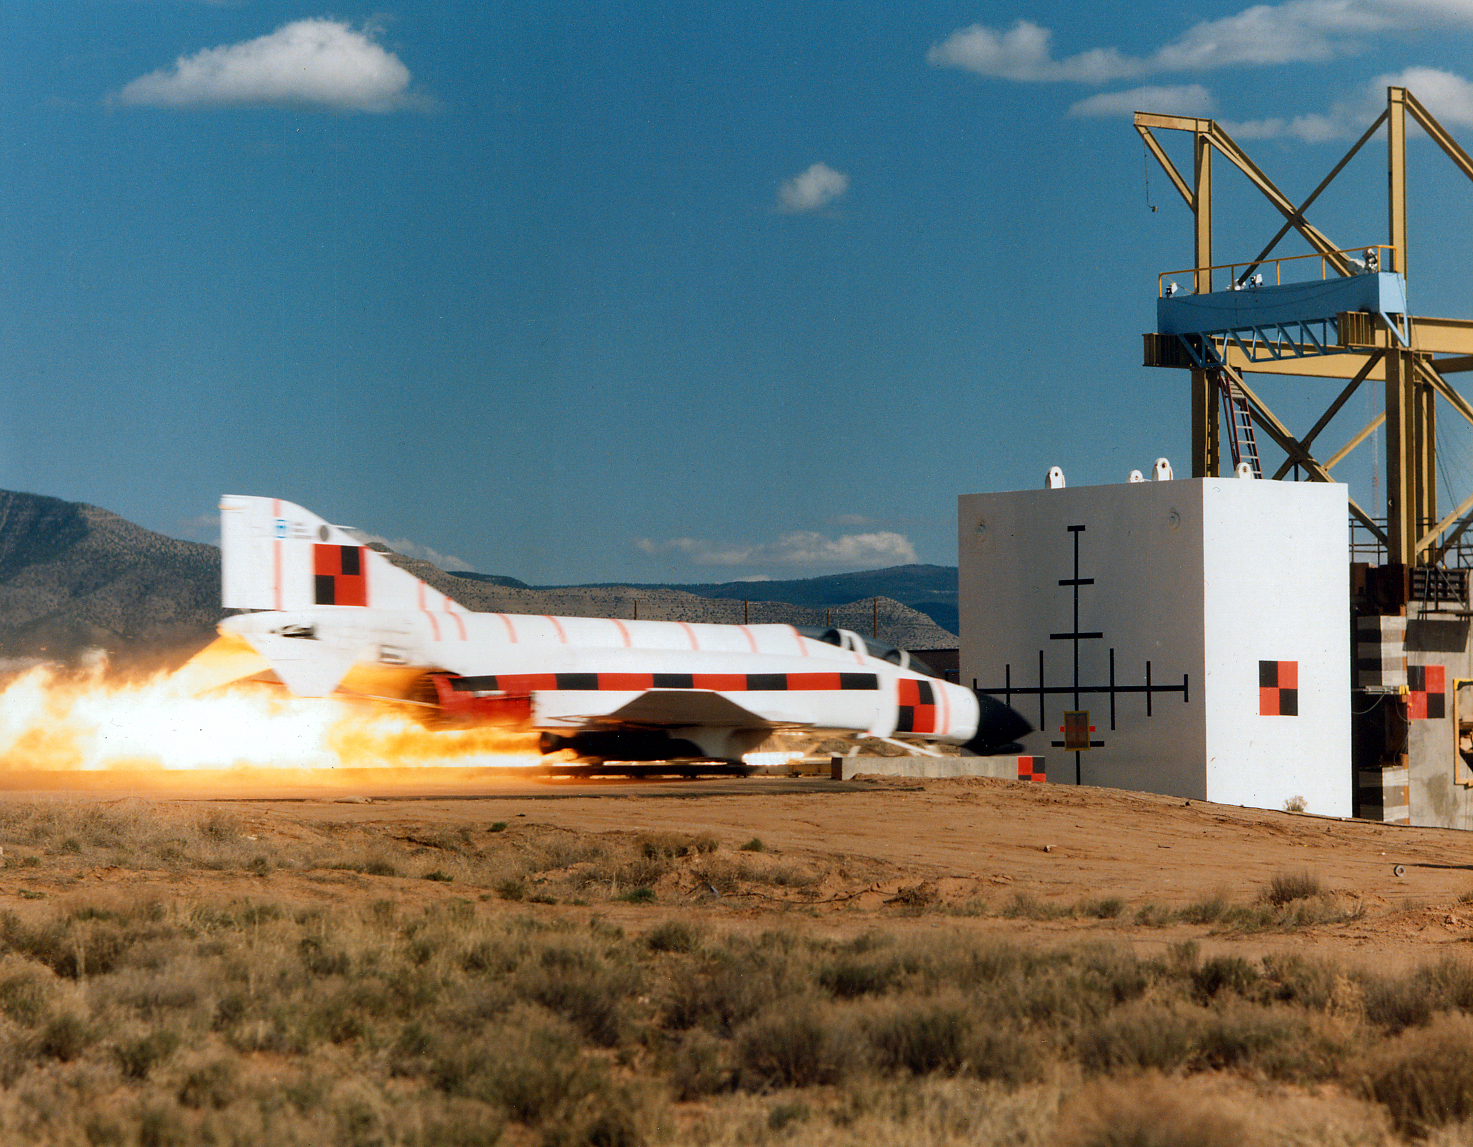
\includegraphics[width=.3\linewidth]{images/Rocket1}
  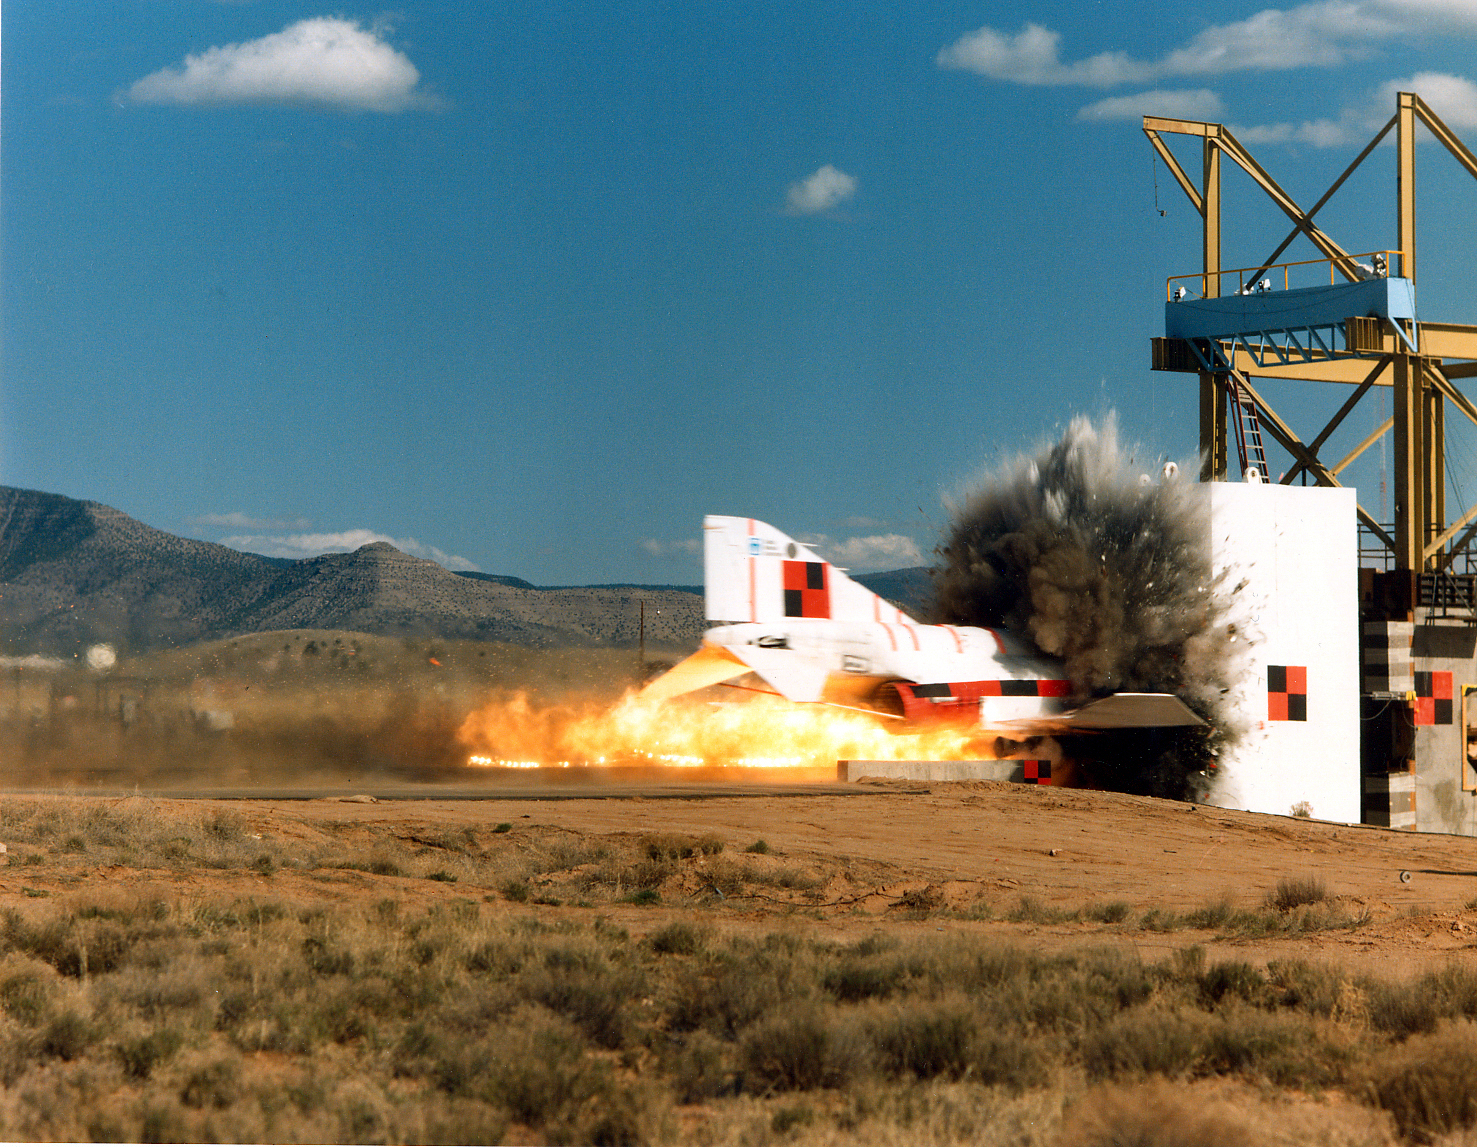
\includegraphics[width=.3\linewidth]{images/Rocket2}
  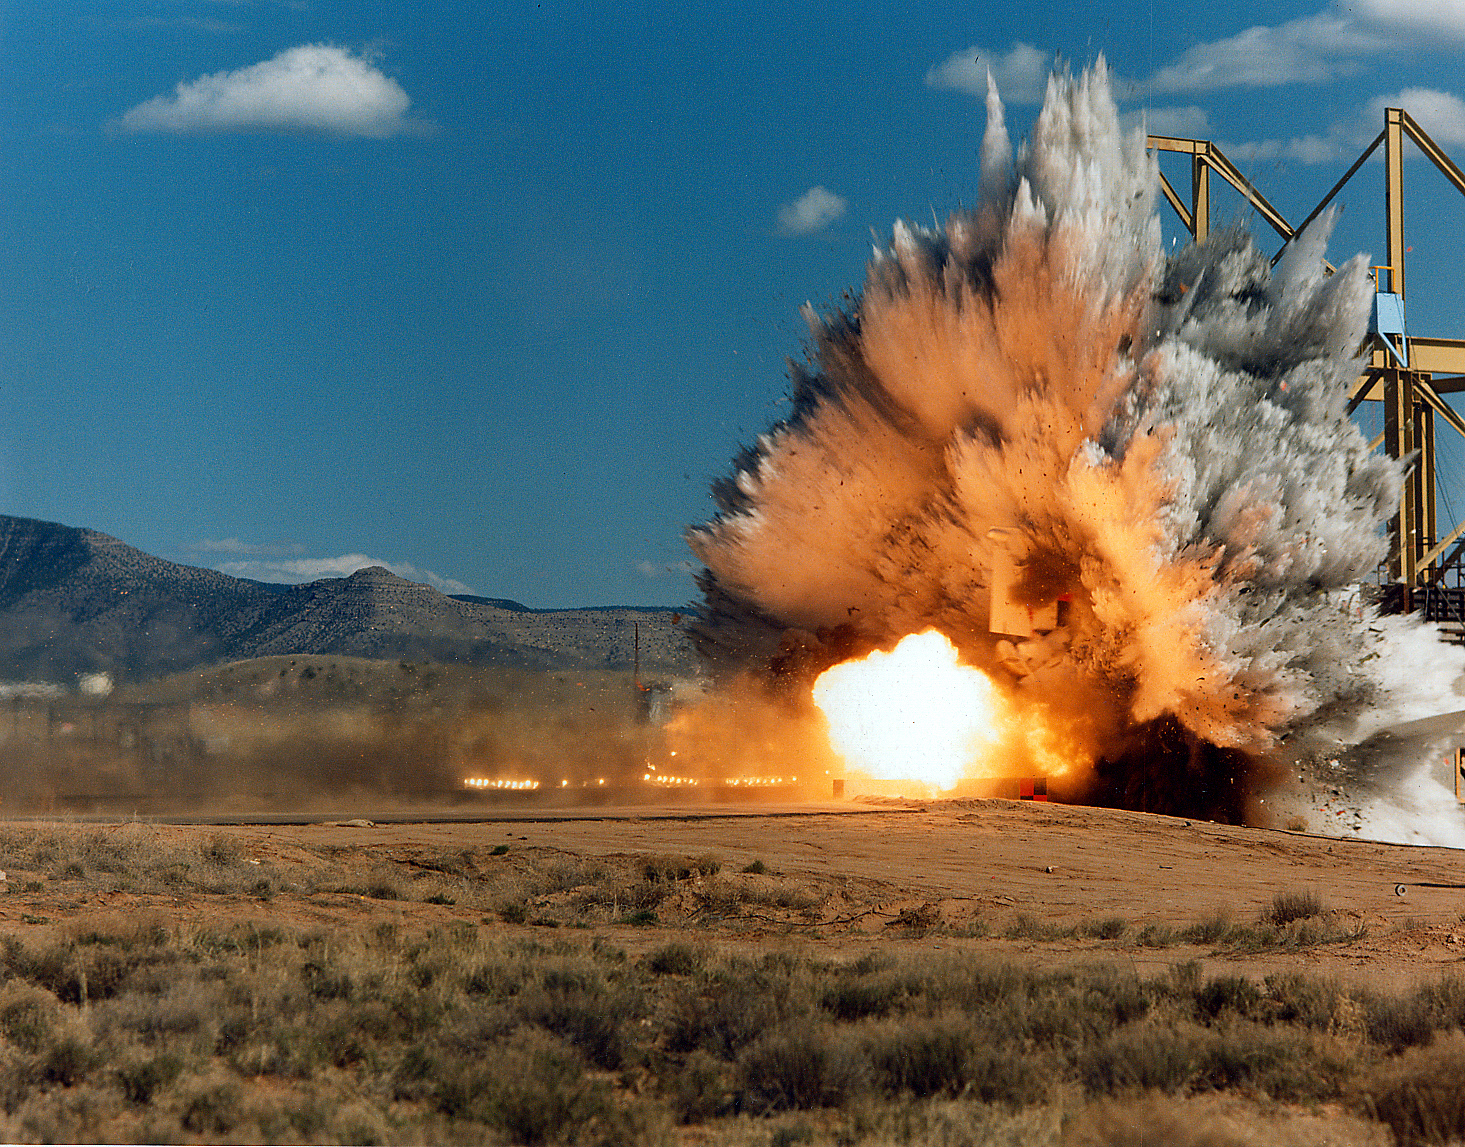
\includegraphics[width=.3\linewidth]{images/Rocket3}
  \caption{This 1988 rocket-sled test has nothing to do with exascale
    computing per se, but it makes for an effective metaphor for the
    ``brick wall'' we anticipate our high-performance computing code to
    collide with.}
  \label{fig:teaser}
}

\begin{document}

\sloppy

\maketitle

\begin{abstract}
The predictions for exascale computing are dire.  Although we have
benefited from a consistent supercomputer architecture design, even across
manufacturers, for well over a decade, recent trends indicate that future
high-performance computers will have different hardware structure and
programming models to which software must adapt.  This paper provides an
informal discussion on the ways in which changes in high-performance
computing architecture will profoundly affect the scalability of our
current generation of scientific visualization and analysis codes and how
we must adapt our applications, workflows, and attitudes to continue our
success at exascale computing.
\end{abstract}

\section{Introduction}
\label{sec:Introduction}

\noindent
Thanks to recent advances in parallel visualization algorithms and
frameworks, we currently benefit from production large-scale
scientific-visualization applications such as ParaView\lcite{ParaView} and
VisIt\lcite{VisIt}, which are shown to be very scalable up to our current
generation of petascale computers\lcite{Childs2010}.  Although the
development of these tools comes from the successful scaling of techniques
originally pioneered over ten years ago\lcite{Ahrens2000,Wylie2001}, recent
trends indicate that future high-performance computers will have different
hardware structure and programming models to which software must adapt.

These grave predictions come from multiple
workshops\lcite{ExascaleArchitecturesReport,ExascaleRoadMap,DARPAExascaleStudy}
where experts convened to discuss the roadmap to building exascale
computers (that is, computers capabile of performing $10^{18}$ floating
point operations per second).  Table~\ref{table:PetascaleVsExascale} gives
a summary comparison between an existing petaFLOP computer and the expected
system performance of a future computer capable of an exaFLOP.  Note that
there is uncertainty in what type of computer architecture will be used to
achieve and exaFLOP (and it is possible different architectures may be used
in different instances).  To compensate for this uncertainty, experts use
the term of design ``swim lanes'' that capture these different approaches.
Two likely swim lanes are captured in
Table~\ref{table:PetascaleVsExascale}.

If all the components of supercomputers were to be scaled uniformly, then
the ``Factor Change'' column in Table~\ref{table:PetascaleVsExascale} would
have uniform values.  However, the factor of change varies wildly from very
small changes to five orders of magnitude.  The main cause for most of this
variability comes from comprimises made to achieve the desired system peak
(the first column of Table~\ref{table:PetascaleVsExascale}) in the
constraints of a limited power budget (the second column of
Table~\ref{table:PetascaleVsExascale}).  DOE has established a power budget
for the exascale machine at 20~MW\lcite{ExascaleArchitecturesReport}.  The
reason for this budget is very pragmatic.  The operating cost of a
supercomputer is roughly \$1 million per megawatt per year.  As such, DOE
determines that it cannot afford more than \$20 million per year to operate
a single supercomputer.  Thus, the challenge of exascale computing is
getting about three orders of magnitude improvement in computation rate
using not much more power than we do today.

\begin{table*}[htdp]
  \centering
  \caption{Comparison of a petascale supercomputer to an expected exascale
    supercomputer\lcite{ScientificDiscoveryExascale2011}.}
  \label{table:PetascaleVsExascale}
  \begin{tabular}{@{}lcccc@{}}
    \toprule
    & & \multicolumn{2}{c}{Exascale (Prediction)} & \\
    System Parameter & Petascale & Swim Lane 1 & Swim Lane 2 & Factor Change \\
    \midrule
    System Peak & 2 Pf/s & \multicolumn{2}{c}{1 Ef/s} & 500 \\
    Power & 6 MW & \multicolumn{2}{c}{$\le$20 MW} & 3\\
    System Memory & 0.3 PB & \multicolumn{2}{c}{32--64 PB} & 100--200 \\ % San Diego report says 50PB
    Total Concurrency & 225K & 1B$\times$10 & 1B$\times$100 & 40,000--400,000 \\
    Node Performance & 125 GF & 1 TF & 10 TF & 8--80\\
    %Node Memory BW & 25 GB/s & 400 GB/s & 4 TB/s & 16 \\
    Node Core Count & 12 & 1,000 & 10,000 & 83--830 \\
    Network BW & 1.5 GB/s & 100 GB/s & 1000 GB/s & 66--660 \\
    System Size (nodes) & 18700 & 1,000,000 & 100,000 & 50--500 \\
    I/O Capacity & 15 PB & \multicolumn{2}{c}{300--1000 PB} & 20--67\\
    I/O BW & 0.2 TB/s & \multicolumn{2}{c}{20--60 TB/s} & 10--30 \\
    \bottomrule
  \end{tabular}
\end{table*}

Using the predictions in Table~\ref{table:PetascaleVsExascale}, this paper
provides an overview of the changes required to our scalable code and how
we use our applications.  In particular, we will note the contrast between
the factor change of related system parameters and discuss the
implications.  This paper provides an informal discussion of these issues.
For a more formal discussion, consult the report from the DOE ASCR 2011
Workshop on Exascale Data Management, Analysis, and
Visualization\lcite{ScientificDiscoveryExascale2011}.

\section{Concurrency}
\label{sec:Concurrency}

\noindent
Let us first compare the amount of memory expected on our exascale machine
with the amount of concurrency programs will have to exhibit at scale.  The
system memory of the machine will grow by a factor of about a hundred,
which is an order of magnitude lower than than the growth of the
computational power.

The reason for this low growth of memory is that memory tends to be power
hungry.  Thus, we simply cannot afford to grow the amount of memory in the
system at a rate equal to the computation.  Furthermore, additional memory
does not directly contribute to the computational rate of the system.  Of
course, by that logic we could create an even cheaper exascale machine by
not adding or perhaps even removing some system memory.  However, doing so
would render the machine useless, and neither DOE nor any other
organization is willing to spend millions of dollars on a useless machine.
So, the amount of memory to be added to an exascale machine is an
engineering decision to maximize the utility of the system while keeping
everything in budget.

In contrast, the total concurrency required by the system will grow by up
to five orders of magnitude.  The reason for this staggering increase in
concurrency is twofold.  First, although Moore's law still holds for the
scaling of the number of transistors (so far), this scaling is no longer
contributing to the faster operation of processing
cores\lcite{ExascaleRoadMap}.  Instead, increased computing power is
achieved by adding more cores to a processor.  Given this fixed calculation
rate per core, we can predict that we will need roughly a million cores to
sustain a rate of $10^{18}$ floating point operations per second.

Of course, the change in Moore's law only accounts for an increase of three
orders of magnitude.  The second factor that is increasing total
concurrency is the interface between the processor and the memory holding
the data it operates on.  Because the latency to off-chip memory is not
expected to improve substantially, practical applications will likely have
to run 10 to 100 threads per core (depending on the type of processor) to
hide this latency by swapping threads during memory
fetches\lcite{ExascaleArchitecturesReport}.  Consequently, a program could
require up to \emph{100 billion concurrent threads} to maintain an
exaFLOP.

\subsection{Scalability of Current Applications}

\noindent
This combination of low memory growth and high concurrency growth
represents serious scaling issues for our parallel high-performance
computation code.  Our current production scientific-visualization
applications use a distributed memory model with a message passing
interface, embodied in the use of MPI\lcite{MPI}, to implement concurrent
processing and communication.  Although this simple but effective model has
served well to the petascale era of supercomputing, it fails to capture
important emerging features in high-performance computing, and it is thus
doomed to break down unless major restructuring efforts are enacted.

To understand why our parallel production applications will fail to scale,
let us consider a simple and artificial but realistic and representitive
example of performing scientific visualization on a regular grid of cells.
For a capability run on the petascale machine represented in
Table~\ref{table:PetascaleVsExascale} we could expect a grid of 1 trillion
cells\lcite{Childs2010}.  On the exascale machine, having about 100 times
more memory, we could expect a grid of 100 trillion cells.

Our current production scientific-visualization applications use MPI to
represent all concurrency, and MPI uses operating system processes to
represent concurrent execution.  Thus, to run on the entirety of a
petascale machine, an application would need about 200 thousand processes
whereas an exascale machine could require up to 100 billion processes.  One
problem with an operating system process is that it is a heavy weight
object.  Associated with each one is an entire program state including a
copy of the machine instructions to be executed.  A library of
general-purpose scientific visualization algorithms could be expected to
run at least 20~MB, and these 20~MB would have to be replicated on each
process.  Replicating this data 200 thousand times on the petascale machine
yields 4~TB, which is a reasonable at less than 2\% of the overall memory
in the system.  However, replicating this data 100 billion times on the
exascale machine yields 2~EB, well over the amount of memory available on
the entire machine (and, incidently, all of its storage).  Thus, we cannot
even start our application on the exascale machine, and that is before we
even load any data.

But let us say we get around that problem, which is an active area of
research\fix{Cite exascale project.}.  Another problem that we run into is
the breakdown of Gustafson's law.  Scientific visualization code, as well
as most modern high-performance parallel code, gets around the limits of
parallel efficiency proposed by Amdahl\lcite{Amdahl1967} by scaling up the
problem size along with the concurrency\lcite{Gustafson1988}.  By
considering a scaled speedup, we can allow the problem size to be an
increasing functionof the number of processes\lcite{Quinn2004}.  However,
limiting the growth of memory limits the scale to which we can grow
problems.

Back to our example, assuming that our visualization algorithm uses data
parallelism, which most modern visualization algorithms
do\lcite{Moreland2012:TVCG}, our 1 trillion cell petascale problem will be
broken into partitions of 5 million cells for each thread.  Experience
shows 5 million cells per thread to be an efficient amount to drive a
visualization pipeline thread\lcite{ParaViewTutorial}.  In contrast, the
equivalent exascale mesh of 100 trillion cells would be divided into
partitions of 1000 cells, a ridiculously small and inefficient amount of
the overhead of a parallel program.

But even ignoring this problem, others abound.  Consider the issue of
adding ghost cells (or sometimes called halo cells) to our partitions.
Ghost cells are critical to the operation of our current parallel
scientific visualization algorithms; they limit the communication required
in the algorithms to make the parallel overhead manageable.  Assuming our
petascale problem is broken into 5 million cell partitions that are roughly
$171^3$ blocks, each block would require $6 \times 171^2$ or about 175
thousand ghost cells.  All total, this is 35 billion ghost cells, which
amounts to about 3.5\% of the original data size.  In contrast, our
exascale mesh would be broken into 1000 cell partitions of $10^3$ blocks,
and each block would require $6 \times 10^2 = 600$ ghost cells.  All total,
this is 60 trillion ghost cells, which amounts to about 60\% of the
original data size.  Growing the memory overhead by 60\% is simply not
feasible in most serious applications.

\subsection{Exascale Programming Challenges}

\noindent

\subsection{Emerging Frameworks for Scientific Discovery at Exascale}

\noindent

\section{Recording Results}
\label{sec:RecordingResults}

\noindent

\subsection{Relative Data Bandwidth}

\noindent

\subsection{Gamut of Coinciding Visualization Solutions}

\noindent

\section{Other Exascale Challenges}
\label{sec:Other}

\noindent

\subsection{Resilience}

\noindent

\subsection{Compression and Extraction}

\noindent

\subsection{Provenance}

\noindent

\subsection{Uncertainty Quantification}

\noindent

\section{Final Remarks}
\label{sec:Conclusion}

\noindent

\section*{Acknowledgments}

\noindent
This report is a summary of ongoing work by a great number collaborators
over many institutions.  In particular, I would like to thank the
following: Nathan Fabian and Ron Oldfield from Sandia National
Laboratories; Kwan-Liu Ma, Robert Miller, and Yecong Ye from the University
of California at Davis; Berk Geveci, Utkarsh Ayachit, Robert Maynard, Brad
King, Andrew C. Bauer, Pat Marion, Sebastien Jourdain, David DeMarle, and
David Thompson at Kitware, Inc.; James Ahrens and Jonathan Woodring at Los
Alamos National Laboratory; Scott Klasky and Norbert Podhorszki at Oak
Ridge National Laboratory; Venkatram Vishwanath, Mark Hereld, and Michael
E. Papka at Argonne National Laboratory; Michel Rasquin and Kenneth
E. Jansen at the University of Colorado at Boulder; Ciprian Docan and
Manish Parashar at Rutgers University.


This work was supported in part by the Director, Office of Advanced
Scientific Computing Research, Office of Science, of the U.S. Department of
Energy under Contract No. 12-015215, through the Scientific Discovery
through Advanced Computing (SciDAC) Institute of Scalable Data Management,
Analysis and Visualization.

This work was supported in part by the DOE Office of Science, Advanced
Scientific Computing Research, under award number 10-014707, program
manager Lucy Nowell.

Sandia National Laboratories is a multi-program laboratory operated by
Sandia Corporation, a wholly owned subsidiary of Lockheed Martin
Corporation, for the U.S. Department of Energy's National Nuclear Security
Administration.

\noindent
{\small SAND 2013-XXXX}

\bibliographystyle{IEEEtranS}
\bibliography{OhShExascale}

\end{document}
